\chapter{Events}  \label{Ch:UGEvents}


In GMAT, events allow a user to determine when 
station contacts, eclipses, or
spacecraft-to-spacecraft occur among others. In general, events are
dependent upon the orbit dynamics and  time dependent parameters,
and therefore can only be determined during or after orbit
propagation.  The implementation of Events requires GMAT to
find the roots of parametric functions of time.  The roots of the
parametric equation are the event times, in the case of a discrete event, or define
the event boundaries, in the case of an interval event.

In this chapter, we'll look at how GMAT calculates the roots of
event functions and hence locates both discrete and interval events. This includes two
subproblems.  The first is determining if a root/event has occurred during
a propagation step.  The second, is determining the numerical value
of the root.  We begin by looking at the
mathematical definition of an event function in GMAT.

\section{Overview of Events}

We begin by defining two types of events: (1) discrete events that occur at
an instant of time, such as the epoch of an impulsive maneuver, and (2) an interval
event that occurs over some finite time span, such as a spacecraft eclipse.  Events are located
using root finding methods.

Let's proceed using an example event.  Assume we wish to determine when a tracking station will next be able to take
measurements of a spacecraft's range and Doppler.  The conditions that must be satisfied, called the event functions,
are that the spacecraft must be 5 degrees above the horizon, and that the relative range rate of the spacecraft must be less than 3 km/s.

1)  Feasible
2)  If not feasible, what condition causes infeasiblity
3)  Ordered for efficiency
4)  Event location of for discrete event 

\begin{equation}
   \Delta t_e < \Delta t_s
\end{equation}

\label{sec:EventFunctionMathDef}

An Event Function in GMAT has three outputs. The general form of an
Event Function is
%
\begin{equation}
    [\hspace{.05 in} \mathbf{f}, \mathbf{d}, \mathbf{p} \hspace{.05 in}] = \mathbf{F} (t, \mathbf{x}(t),\mathbf{C}
    ) \label{Eq:GeneralEventFunction}
\end{equation}
%
where $t$ is the current time, $\mathbf{x}(t)$ is a vector of time
dependent parameters such as spacecraft states, and $\mathbf{C}$ is
a vector of constants.  $\mathbf{f}$ is vector of function values at
$t$, $\mathbf{d}$ is a vector describing the or sign change we wish
to track that occurs at the root, and $\mathbf{p}$ is a vector that
tells GMAT whether a root is possible or not.  Let's talk about some
of the output variables in more detail.

For efficiency and convenience, the user can calculate several
different function values, $f$, inside of a single event function,
$\mathbf{F}$. This is useful when several functions require similar
yet expensive calculations.  GMAT allows the user to pass back a
vector of function values in the output parameter $\mathbf{f}$,
where the components of $\mathbf{f}$ are simply the values of the
different functions $f$, or
%
\begin{equation}
     \mathbf{f} = [ \hspace{.05 in} f_1(t, \mathbf{x}(t),\mathbf{C}),  f_2(t,
     \mathbf{x}(t),\mathbf{C}) ... f_n(t,
     \mathbf{x}(t),\mathbf{C})\hspace{.05 in}]^T
\end{equation}
%
The output parameter $\mathbf{d}$ allows
the user to define which type of roots for GMAT to calculate. For
example, in some cases  we might only be interested in roots that
occur when the function changes from a negative value to a positive
value. In other situations we may only be interested in roots that
occur when the function passes from positive to negative. Finally,
we may be interested in both types of roots.  $\mathbf{d}$ is a
vector that has the same number of elements as $\mathbf{f}$, and the
first element  of $\mathbf{d}$ corresponds to the first element of
$\mathbf{f}$ and so on. Table \ref{Table:EventFunction_dValues}
summarizes the allowable choices for components of $\mathbf{d}$ and
the action GMAT will take depending upon the selection.
%
\begin{table}[htb]
\caption{ Allowable Values for $\mathbf{d}$ in Event Function
Output}
\begin{tabular}{p{.5 in} p{2.5 in}}
   \hline
   Value & Action\\
   \hline \hline
     d = 1 & Find roots when the function is moving  in the positive
    direction. \\
    d = -1 & Find roots when the function is moving in the
        negative
    direction. \\
   d = 2 & Find both types of roots\\
   \hline
 \end{tabular}
 \label{Table:EventFunction_dValues}
\end{table}

The last output variable in the Event Function output, $\mathbf{p}$,
is a flag that allows the user to tell GMAT whether or not a root is
possible.  If a component of $\mathbf{p}$ is zero, then GMAT will
not attempt to try to find a root of the corresponding function in
$\mathbf{f}$.  This flag is included to improve the efficiency of
the algorithm. It is often possible to perform a few simple
calculations to determine if a root is possible or not. For example,
let's assume an event function is written to track Earth shadow
crossings and that the function is positive when a spacecraft is not
in Earth's shadow, and negative when it is in Earth shadow.  It is a
relatively simple calculation to determine if a spacecraft is on the
day-side of Earth by taking the dot product of the Sun vector and
the spacecraft's position vector. If the quantity is positive, there
is no need to continue calculating the actual function value.

Now that we've looked at the definitions of the inputs and outputs
of an Event Function, let's look at some different approaches to
finding the roots of an event function.


\section{Issues in Locating Zero Crossings}

Before discussing the practical issues in finding roots of Event
Functions, let's take a look at a hypothetical function to
illustrate some of the issues that must be addressed. Figure
\ref{fig:SampleEventFunction} shows a sample event function.  The
smooth line represents the locus of points of the function itself,
and the large ``X" marks represent the function values at the
integration time steps.  The smaller tick marks indicate the
function values at the internal integrator stages, which may be
available if we use a dense output numerical integrator.

In general, we don't have continuous time expressions for the inputs
to event functions.  We only know the inputs to Event Functions at
discrete points in time, so we only know the Event Function values
at discrete points in time.  Since these discrete times come from
the numerical integration of a differential equation, we can only
calculate Event Function values at the integration time steps, or at
the internal stages if the information is available.  This fact can
cause a significant problem because an Event Function may vary
rapidly and the discrete times at which we know the Event Function
may not give an accurate picture of the function.

Let's consider a few ways in which we can determine if a root has
occurred, given a set of times and Event Function values.  The most
obvious method is to simply look for sign changes in the function
values. If the function changes sign, then we know we have bracketed
a root. This approach will incorrectly conclude that a zero crossing
did not occur, if there is an even number of zero crossings between
two function values.  Another approach is to fit a polynomial
through the data, and see if the polynomial has any real roots.
While this approach may be more accurate than looking for sign
changes in some cases, it still does not guarantee a zero crossing
is missed. A third approach might be to force the integrator to
select step sizes based on the rate of change of the Event Function.
We will not investigate this method further here though.

In short, there is no way to guarantee that a root crossing is
missed.  However, by having an understanding of the Event Function,
having control over the maximum integration step size, and having
access to the internal integrator stages when using a dense output
integrator, we can do a acceptably good job determining when
zero-crossings occur.  Once a zero-crossing is identified, there are
well known ways to calculate the actual root value.




\begin{figure*}[htb]
    \centering
    %\begin{picture}(130,120)(140,0)
        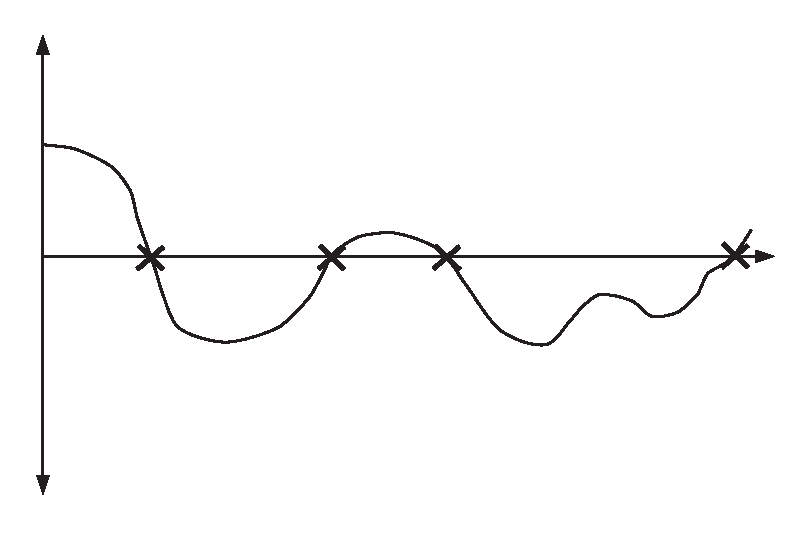
\includegraphics[scale=1.0]{Images/EventsFunction.eps}
   % \end{picture}
    \caption{ Sample Event Function Output }
    \label{fig:SampleEventFunction}
\end{figure*}

\begin{equation}
    \mathbf{F} = \mathbf{F} (t, \mathbf{x}(t),\mathbf{C}   )
\end{equation}
%
We want to find all $t$ such that
%
\begin{equation}
    \mathbf{F} (t, \mathbf{x}(t),\mathbf{C}   ) = 0
\end{equation}


\section{Root Finding Options in GMAT}

In implementing a root finding approach, we need to balance accuracy
and the need to find every root, with speed and performance.  One
way to do this is to allow the user to select between different
approaches depending upon the accuracy needed for a particular
application.   The user has several controls to tell GMAT how to
determine if a zero crossing has occurred, and how to calculate the
numerical value of a root if one has been detected. Let's look at
the choices implemented in GMAT, and discuss some options that can
be included if a more robust method is required.

The first group of controls available to the user are related to how
or if GMAT tries to determine if a root has occurred.  The user can
provide a flag in the output of an Event Function that tells GMAT
whether it is possible that a root has occurred during the last
integration step. This flag is notated as $\mathbf{p}$ and is
discussed in section \ref{sec:EventFunctionMathDef}.  If an element
of $\mathbf{p}$ is zero, then GMAT will not use more sophisticated
and therefore more computationally intensive methods to determine if
a zero crossing for the particular component of the event function
has occurred.  $\mathbf{p}$ can be either zero or one, and can
change value during propagation.  If $\mathbf{p}$ changes from zero
to one, GMAT begins using a root checking method specified by the
user to determine if a zero crossing has occurred, and begins
storing function data  in case it is needed to interpolate a root
location.

The second control that determines if a  zero crossing has occurred
is called \st{RootCheckMethod} in the GMAT script language.  There
are several RootCheckMethod options available and the user can
currently select between \st{FunctionSignChange} and
\st{PolynomialFit}.  If the user selects \st{FunctionSignChange},
then GMAT looks for sign changes in the function output to determine
if a zero crossing has occurred.  If the user selects
\st{PolynomialFit}, then GMAT fits a polynomial to the Event
Function data, and checks to see if the polynomial has any real
roots. If the polynomial has real roots, then a zero crossing has
occurred. The type of polynomial GMAT uses in \st{RootCheckMethod}
is the same as it uses in \st{RootFindingMethod} and is discussed in
more detail below.

If a zero crossing is detected, there are many ways to determine the
numerical value of the root.  The user can select between the
different methods by using the \st{RootSolvingMethod} option. The
two methods currently implemented in GMAT are called
\st{QuadraticPolynomial} and \st{CubicSpline} in the GMAT script
language.  As the name suggests, if the user selects
\st{QuadraticPolynomial}, then GMAT uses the last three function
values to create a quadratic polynomial.  Then, the quadratic
equation is used to determine the root locations. Similarly, if the
user selects \st{CubicSpline}, GMAT constructs a cubic spline and
then uses interpolation to find the root value.

Allowing the options above requires that care is taken in designing
an algorithm to track events.  In the next section we discuss some
of the issues that must be addressed in the Event Function
algorithm, and present a flow chart that describes the algorithm in
detail

\section{Algorithm for Event Functions }


\begin{table}[htb]
\caption{ Variables in Event Function Algorithm}
\begin{tabular}{p{.5 in} p{2.5 in}}
   \hline
   Variable & Definition\\
   \hline \hline
    $n_r$     & Number of data points required to use the requested \st{RootSolvingMethod} option \\
    $n_c$     & Number of data points required to use the requested \st{RootCheckMethod} option\\
    $\mathbf{f}$  & A vector of function values provided by the user
    defined Event Function\\
    $N$           &  The length of $\mathbf{f}$, which is the number
    function values contained in  the output of a user defined Event
    Function.\\
    $\mathbf{d}$   &  A vector of flags (length $N$) that defines which
    type of roots to track.  (negative to positive, positive to
    negative, or both)\\
    $\mathbf{p}$   &  A vector of flags (length $N$) that tells whether or not a
    zero crossing is possible.  A component of $\mathbf{p}$ is one
    if a root is possible, otherwise it is zero.\\
    $\mathbf{Startup}$ & A vector of flags of lenght $N$.  The components of $\mathbf{Startup}$ correspond to the components of $\mathbf{f}$.
                        A component of $\mathbf{Startup}$ is one, if there is
                       less than max($n_r$,$n_c$) data points saved for use in root finding.
                        Otherwise, a component of $\mathbf{Startup}$ is zero.\\
   \hline
 \end{tabular}
 \label{Table:VariablesinEventFunctionChart}
\end{table}



\clearpage
\begin{figure*}[htb]
    \centering
    \begin{picture}(0,400)(310,300)
        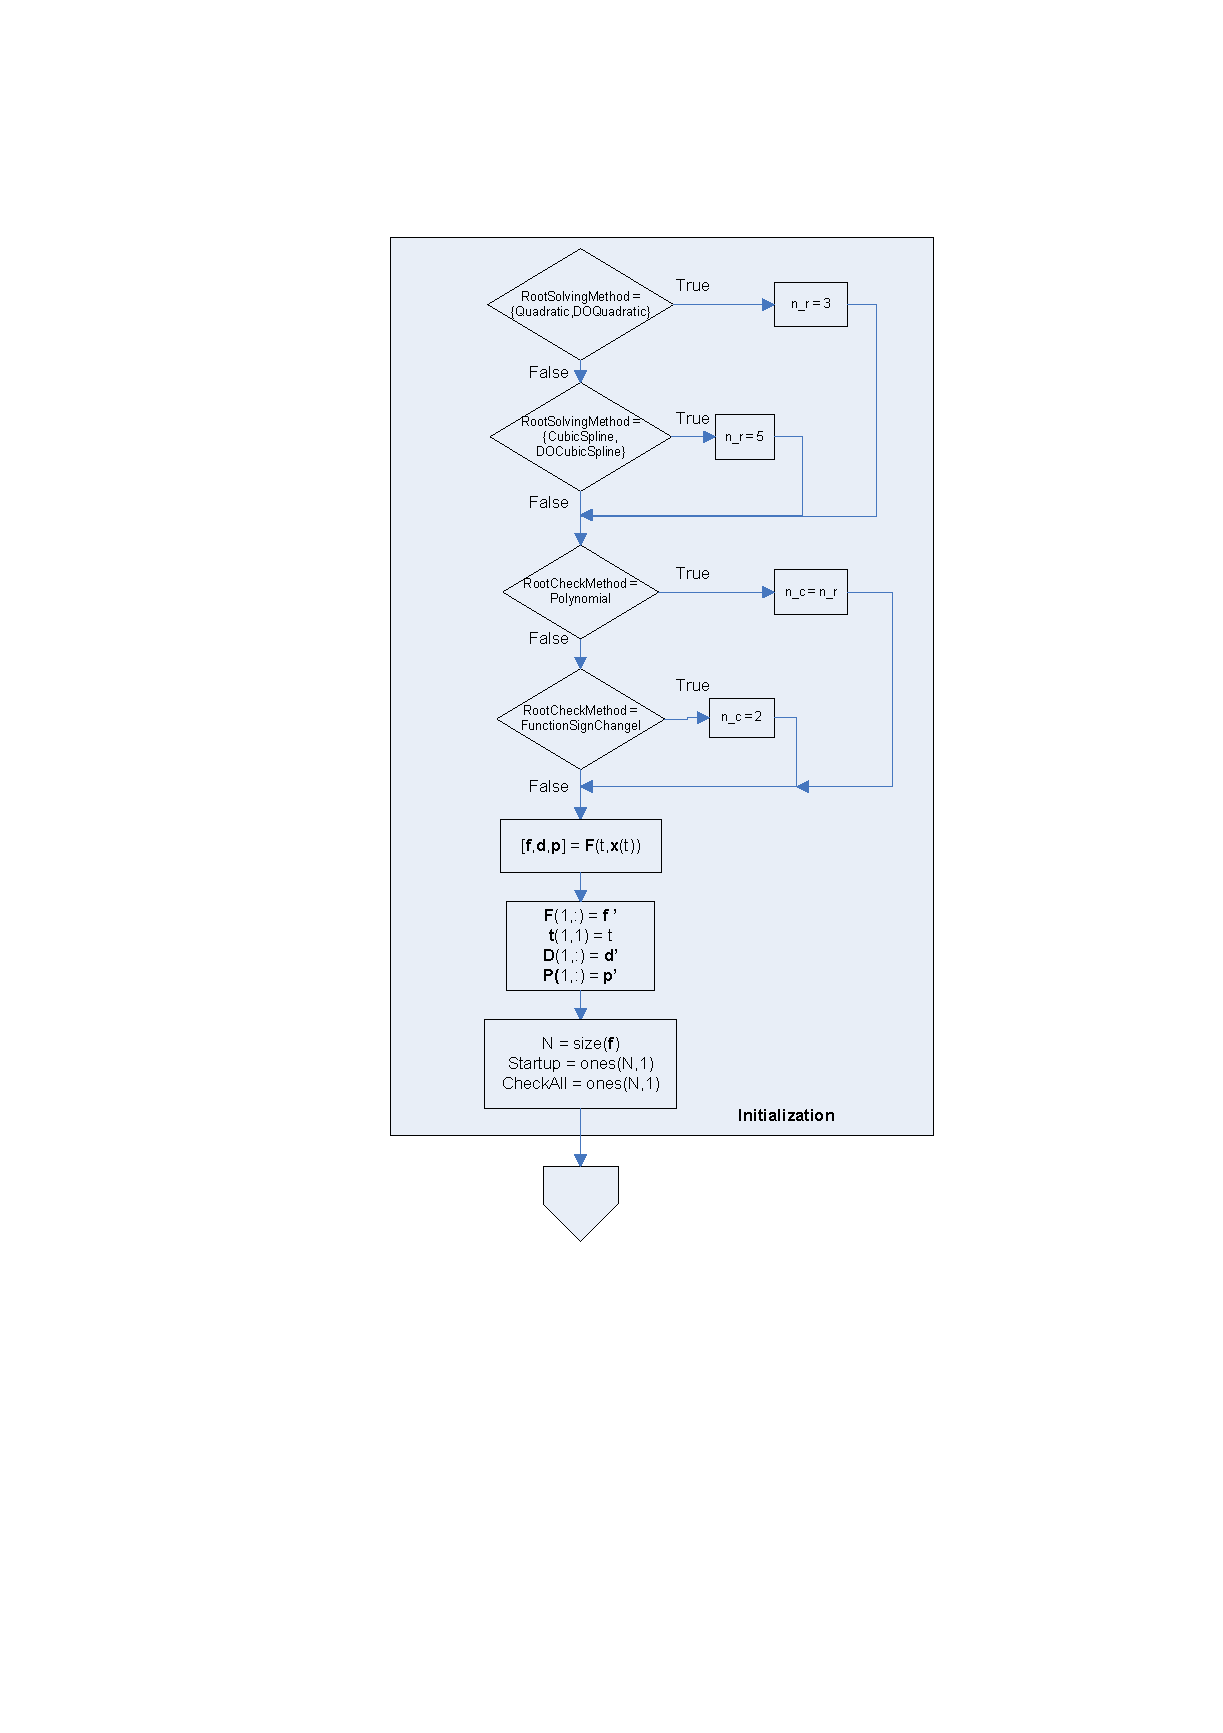
\includegraphics[scale = 1.0]{Images/EventFunctionsFlowChart.eps}
    \end{picture}
    \vspace{1 in}
    \caption{ Initializations for the Event Location Algorithm }
    \label{Plot:EventFunctionsFlowChart}
\end{figure*}

\clearpage
\begin{figure*}[htb]
    \centering
    \begin{picture}(0,400)(265,210)
        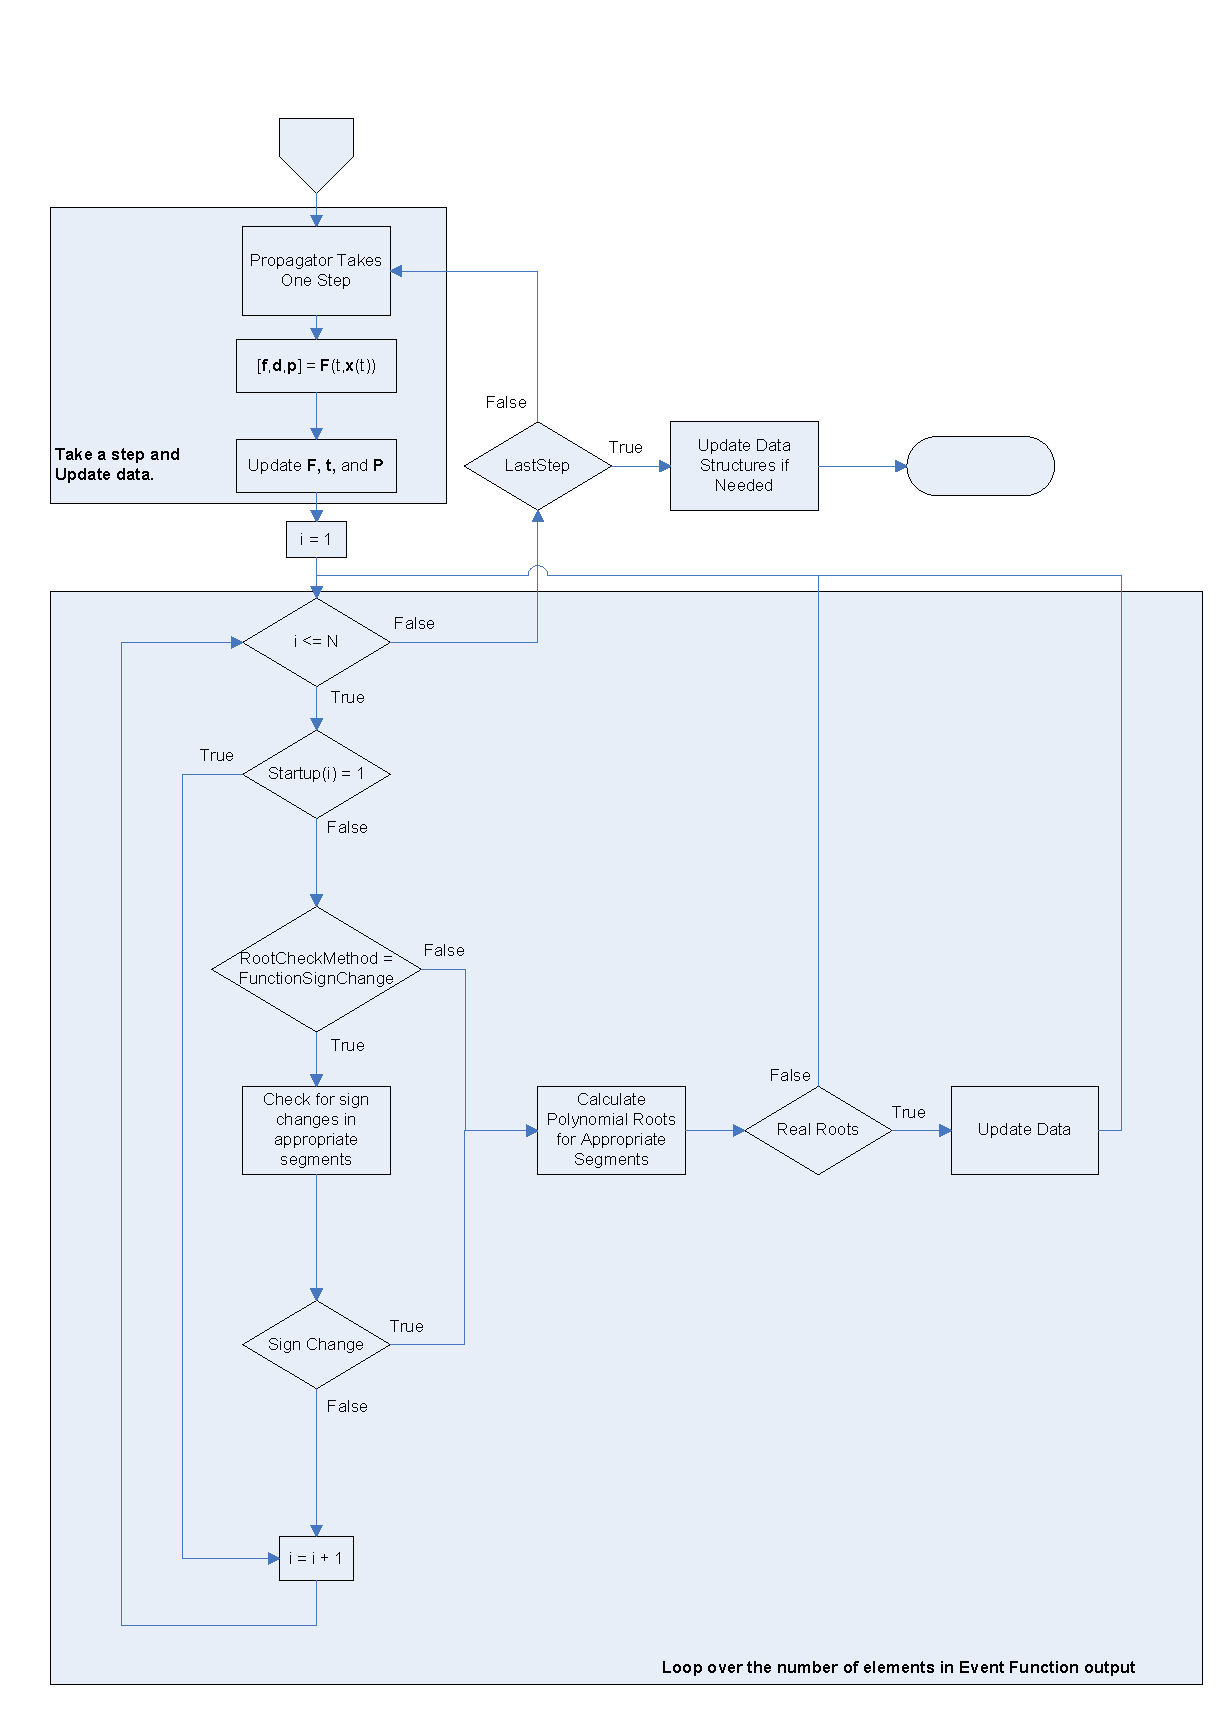
\includegraphics[scale = .9]{Images/EventFunctionsFlowChart2.eps}
    \end{picture}
    \vspace{1 in}
    \caption{ Event Location Algorithm }
    \label{Plot:EventFunctionsFlowChart2}
\end{figure*}
